
Unphysical asymptotic charge density decays occasionally arise in the
\isa 
procedure due to basis set incompleteness and numerical instabilities. These
unphysical decays can
skew optimization of \isa-based exponents, $B_i^{ISA}$, and need to be corrected.
Generally speaking, there exists some range of distances in the valence region
that \emph{does} exhibit the expected exponential decay; we extrapolate the
decay from this intermediate region to describe the asymptotic region using
the following algorithm:

\begin{enumerate}

\item Take the log of each atomic density (henceforth logdens) to linearize
the asymptotic density.
\label{step1}
\item Compute the 2\super{nd} derivative of logdens. This can be
done analytically, as the \isa procedure outputs an analytical expression (in
terms of Gaussian basis functions) for the atomic density.
\label{step2}
\item Determine the `intermediate region' of exponential decay by locating the
largest range where the 2\super{nd} derivative of logdens is zero
to within a fixed tolerance.  Here we utilize a tolerance of 0.3 a.u. (absolute cutoff)
or 190\% of the smallest exponent in the Gaussian basis set (relative cutoff),
whichever is smaller.  
The latter cutoff accounts for the eventual asymptotic Gaussian-type decay
dictated by the smallest $\zeta$ in the ISA basis.
The endpoints of this intermediate region are denoted $r1$ and $r2$, respectively.
\item Calculate the slope $m$ and intercept $b$ for the line defined by
$r1$, $r2$, and their respective values of logdens. 
\label{step3}
\item Replace all values of logdens after $r2$ with $mr + b$.  The resulting
atomic density is labeled in the main text as `Asymptotically-corrected ISA
densities'.
\label{step4}

\end{enumerate}

A visual of these steps is shown in \ref{fig:acetone-extrapolation}.


    %%%%%%%%% Bij Combination Rule %%%%%%%%%%%
    \begin{figure}
    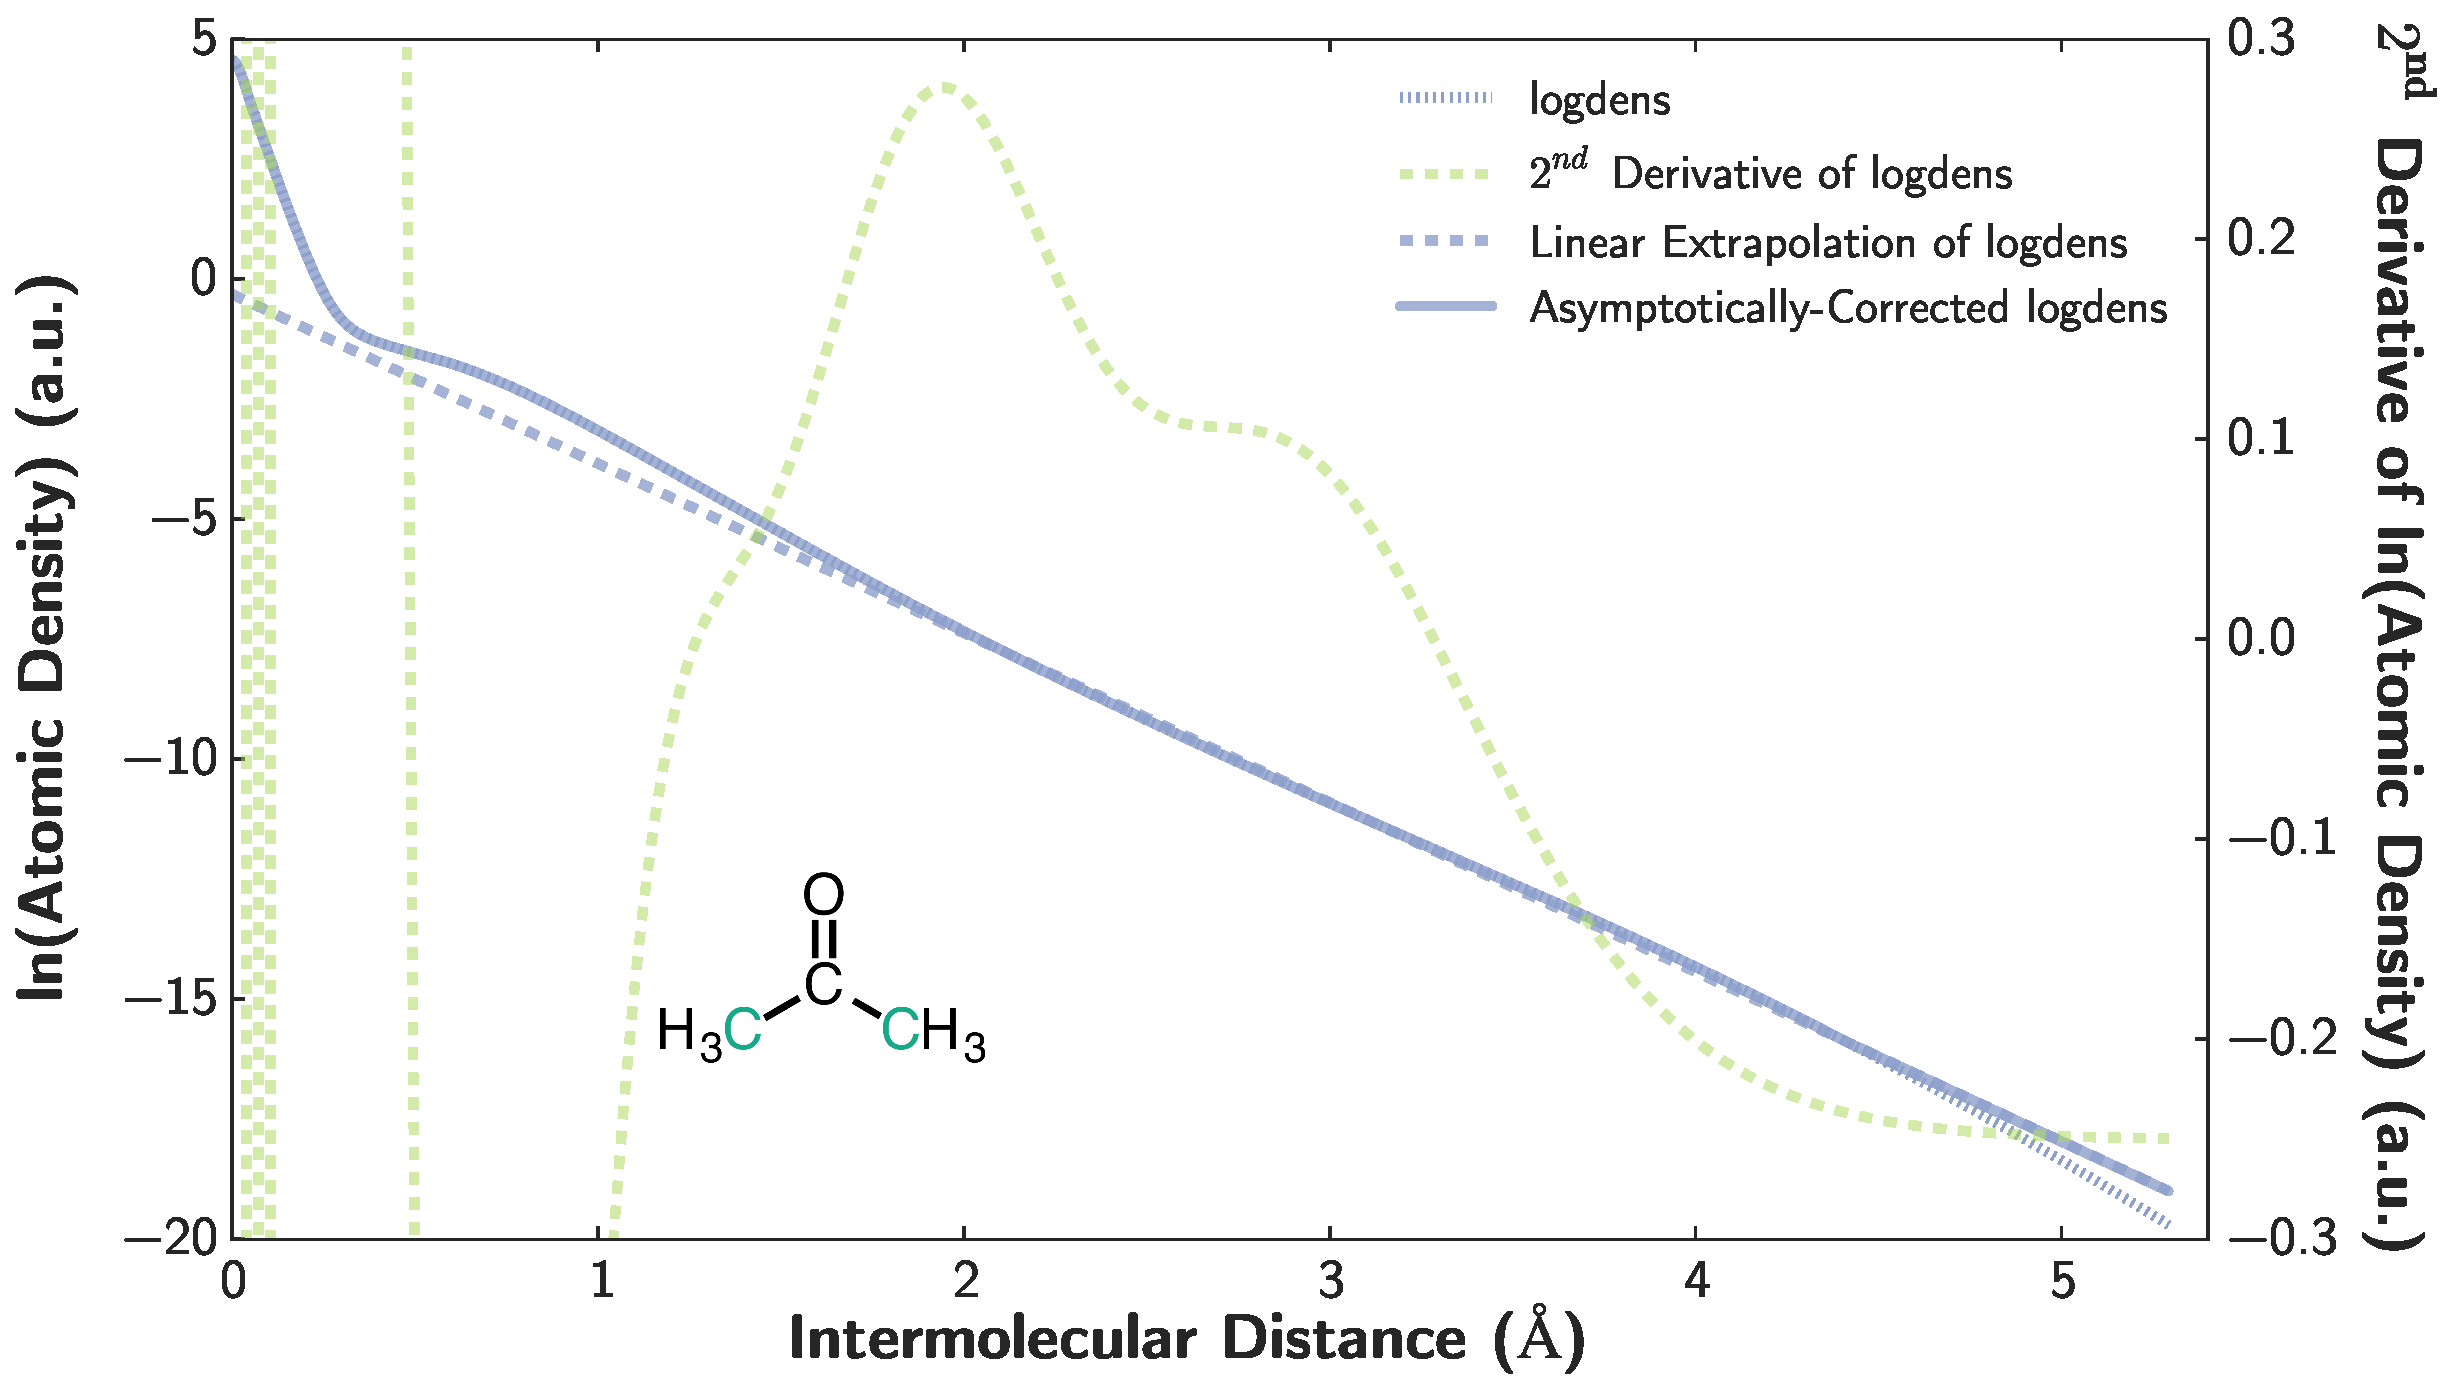
\includegraphics[width=0.9\textwidth]{workflow/acetone_extrapolation.pdf}
    \caption
        [Linear extrapolation algorithm for the methyl carbon in acetone.]
        {
        Linear extrapolation algorithm for the methyl carbon in acetone.
Depicted are (in legend order) Steps \ref{step1}, \ref{step2}, \ref{step3},
and \ref{step4} in the extrapolation algorithm. Note that some portions of the
$2^{nd}$ derivative extend off the graph; also note that most of logdens
is located underneath the asymptotically-corrected curve.
           		  }
    \label{fig:acetone-extrapolation}        
    \end{figure}
    %%%%%%%%% Bij Combination Rule %%%%%%%%%%%



